\subsection{Subarreglo máximo (Kadane)}

Recuérdese el problema del \hyperref[sec:subarreglo_max]{subarreglo máximo}, ya presentado en la sección de dividir y conquistar: dado un arreglo con \(n\) números \([a_0, a_1, \ldots, a_{n-1}]\), hallar los índices \(i\), \(j\) tales que la suma \(\sum_{k=i}^j a_k\) sea máxima. Esta sección aborda el mismo problema mediante programación dinámica.

\subsubsection{Propiedades}

El problema presenta subestructura óptima: la suma máxima de un subarreglo que termina en el índice \(i\) se construye a partir de la suma máxima de un subarreglo que termina en \(i-1\), como se detalla a continuación.

\subsubsection{Modelo}

Se define el estado \(f(i)\) como la suma del subarreglo máximo que termina exactamente en el índice \(i\), es decir, que incluye a \(a_i\) como su último elemento.

Para \(i = 0\), el único subarreglo que termina ahí es el que contiene solo a \(a_0\), por lo que \(f(0) = a_0\). Para \(i > 0\), hay dos formas de construir un subarreglo que termine en \(i\): extender el subarreglo máximo que termina en \(i-1\) añadiéndole \(a_i\), o empezar de nuevo en \(i\), descartando lo anterior. Se elige la que dé mayor suma:
\[
f(i) = \begin{cases}
  a_0 & \text{si } i = 0. \\
  \max\{a_i,\ f(i-1) + a_i\} & \text{si } i > 0.
\end{cases}
\]
La respuesta al problema no es \(f(n-1)\), sino el máximo entre todos los estados, \(\max_{0 \leq i < n} f(i)\), pues el subarreglo máximo puede terminar en cualquier índice del arreglo.

A partir de la relación de recurrencia, el grafo de dependencias es una cadena: cada vértice \(i\) depende únicamente de \(i-1\), sin más arcos entrantes.

\begin{center}
\setbox0=\hbox{%
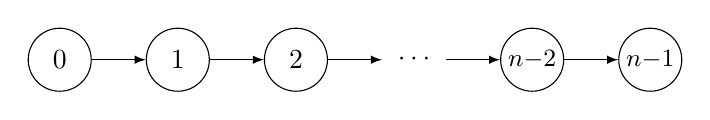
\begin{tikzpicture}[
  vertex/.style={circle, draw, minimum size=0.8cm, inner sep=0pt},
  vertexn/.style={circle, draw, minimum size=0.8cm, inner sep=1pt, font=\small},
  hidden/.style={circle, draw=none, minimum size=0.8cm, inner sep=0pt},
  -latex,
]
  \node[vertex] (f0) at (0, 0) {0};
  \node[vertex] (f1) at (1.5, 0) {1};
  \node[vertex] (f2) at (3, 0) {2};
  \node[hidden] (f3) at (4.5, 0) {$\cdots$};
  \node[vertexn] (fnm2) at (6, 0) {$n{-}2$};
  \node[vertexn] (fnm1) at (7.5, 0) {$n{-}1$};

  \draw (f0) -- (f1);
  \draw (f1) -- (f2);
  \draw (f2) -- (f3);
  \draw (f3) -- (fnm2);
  \draw (fnm2) -- (fnm1);
\end{tikzpicture}%
}
\ifdim\wd0>\textwidth
  \resizebox{\textwidth}{!}{\copy0}
\else
  \makebox[\linewidth]{\copy0}
\fi
\captionof{figure}{Grafo de dependencias del subarreglo máximo.}
\label{fig:kadane_grafo_dependencias}
\end{center}
